\documentclass[tikz,border=12pt]{standalone}
\usepackage[T1]{fontenc}
\usepackage{mathpazo}
\usepackage{amsmath,amssymb}
\usetikzlibrary{arrows.meta, positioning, calc, fit}

\definecolor{stblue}{HTML}{7B97AD}
\definecolor{rwgold}{HTML}{B8995E}
\definecolor{sage}{HTML}{7A9A7E}
\definecolor{dkbrown}{HTML}{3D3530}
\definecolor{wmgray}{HTML}{7B7067}
\definecolor{cream}{HTML}{F9F6F0}
\definecolor{border}{HTML}{D4C9B8}
\definecolor{terracotta}{HTML}{C47A6A}
\definecolor{lavender}{HTML}{907EA0}

\begin{document}
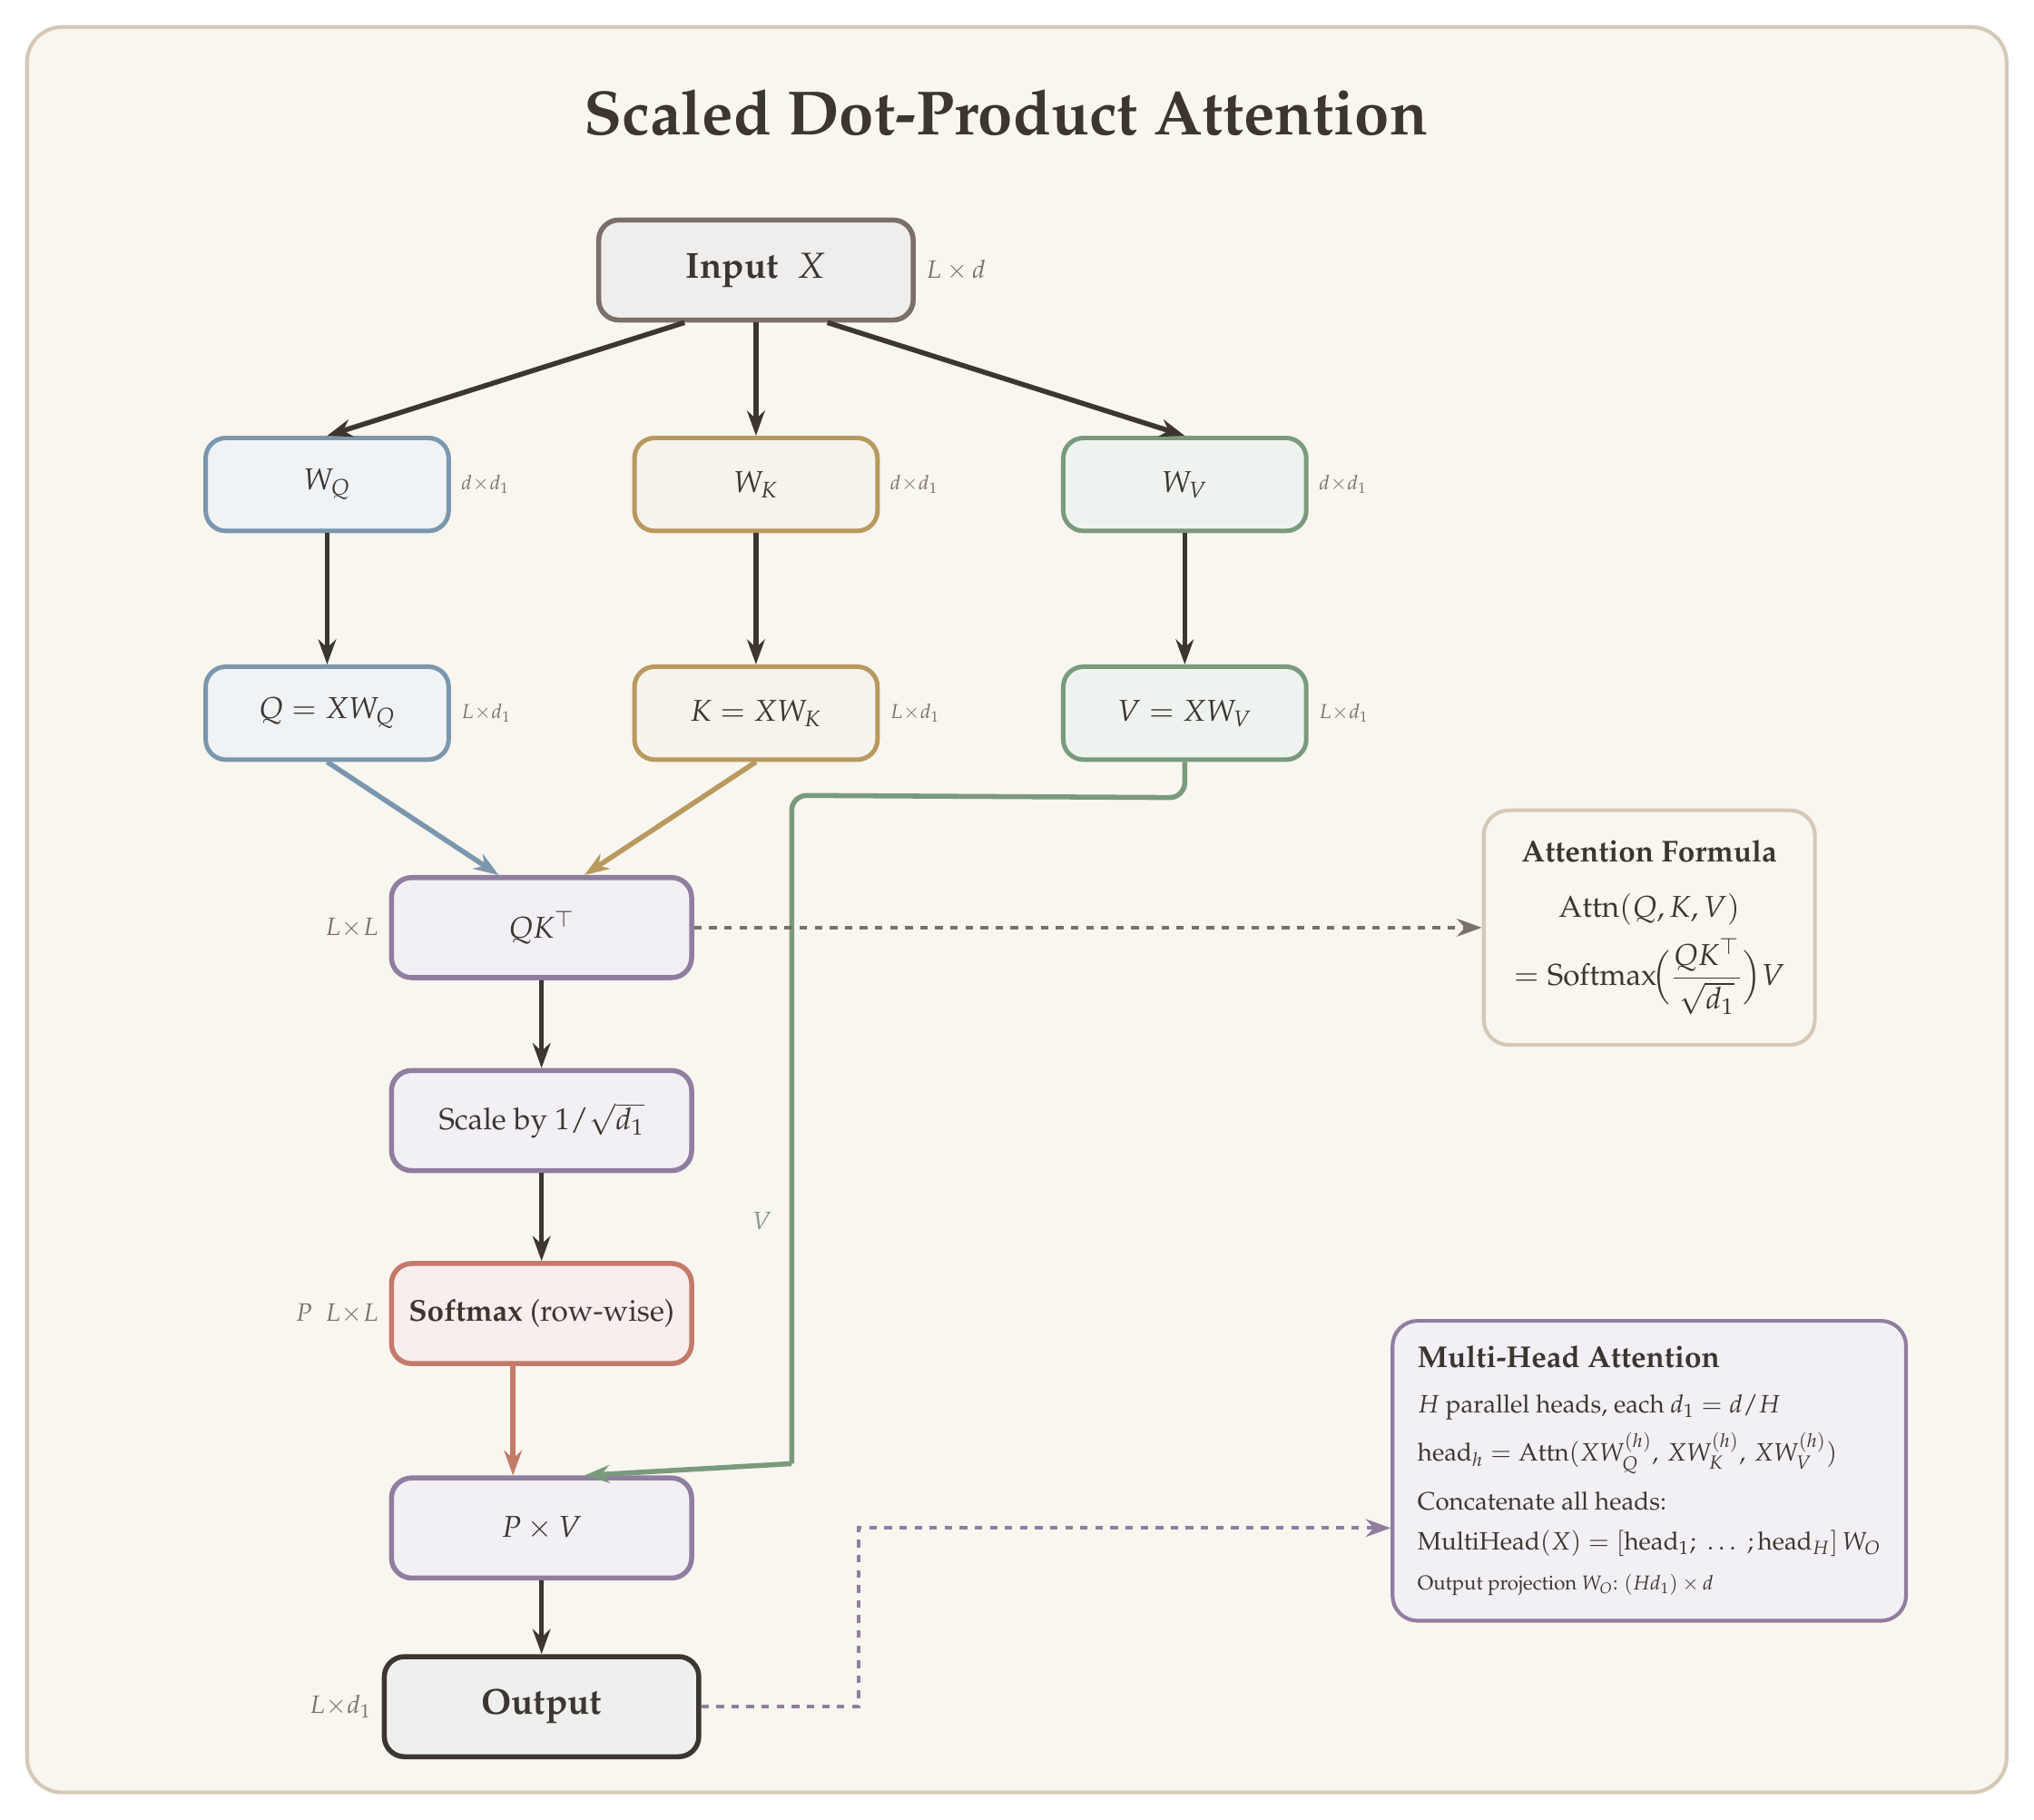
\begin{tikzpicture}[
  >={Stealth[length=3.5mm, width=2.5mm]},
  opbox/.style={
    draw=#1, line width=2pt, fill=#1!12, rounded corners=8pt,
    minimum width=42mm, minimum height=14mm, font=\large, text=dkbrown,
    align=center, inner sep=6pt
  },
  projbox/.style={
    draw=#1, line width=1.8pt, fill=#1!12, rounded corners=8pt,
    minimum width=34mm, minimum height=13mm, font=\large, text=dkbrown,
    align=center, inner sep=5pt
  },
  dimlab/.style={
    font=\footnotesize, text=wmgray, inner sep=1pt
  },
  arr/.style={->, line width=2pt, dkbrown},
  lbl/.style={font=\normalsize, text=wmgray, align=center, fill=cream, inner sep=2pt},
]

% Background
\fill[cream, rounded corners=14pt] (-7.2,-22.5) rectangle (20.5,2.2);
\draw[border, rounded corners=14pt, line width=1.5pt] (-7.2,-22.5) rectangle (20.5,2.2);

% Title
\node[font=\Huge\bfseries, text=dkbrown] at (6.5,1.0)
  {Scaled Dot-Product Attention};

% =============================================
% TOP: Input X
% =============================================
\node[draw=wmgray, line width=2pt, fill=wmgray!12, rounded corners=8pt,
      minimum width=44mm, minimum height=14mm,
      font=\Large, text=dkbrown, align=center, inner sep=6pt]
  (input) at (3,-1.2)
  {\textbf{Input}\; $X$};
\node[dimlab, font=\normalsize, right=3pt of input.east] {$L \times d$};

% =============================================
% Projection matrices: W_Q, W_K, W_V
% =============================================
\node[projbox=stblue] (wq) at (-3,-4.2) {$W_Q$};
\node[dimlab, right=3pt of wq.east] {$d \!\times\! d_1$};

\node[projbox=rwgold] (wk) at (3,-4.2) {$W_K$};
\node[dimlab, right=3pt of wk.east] {$d \!\times\! d_1$};

\node[projbox=sage] (wv) at (9,-4.2) {$W_V$};
\node[dimlab, right=3pt of wv.east] {$d \!\times\! d_1$};

% Arrows: X -> projections
\draw[arr] ([xshift=-10mm]input.south) -- (wq.north);
\draw[arr] (input.south) -- (wk.north);
\draw[arr] ([xshift=10mm]input.south) -- (wv.north);

% =============================================
% Q, K, V results
% =============================================
\node[projbox=stblue] (Q) at (-3,-7.4)
  {$Q = X W_Q$};
\node[dimlab, right=3pt of Q.east] {$L \!\times\! d_1$};

\node[projbox=rwgold] (K) at (3,-7.4)
  {$K = X W_K$};
\node[dimlab, right=3pt of K.east] {$L \!\times\! d_1$};

\node[projbox=sage] (V) at (9,-7.4)
  {$V = X W_V$};
\node[dimlab, right=3pt of V.east] {$L \!\times\! d_1$};

% Arrows: projections -> Q,K,V
\draw[arr] (wq.south) -- (Q.north);
\draw[arr] (wk.south) -- (K.north);
\draw[arr] (wv.south) -- (V.north);

% =============================================
% MIDDLE: Computation flow (all centered at x=0)
% =============================================

% Step 1: Q K^T
\node[opbox=lavender] (matmul1) at (0,-10.4)
  {$Q K^\top$};
\node[dimlab, font=\normalsize, left=3pt of matmul1.west] {$L \!\times\! L$};

\draw[arr, stblue] (Q.south) -- ([xshift=-6mm]matmul1.north);
\draw[arr, rwgold] (K.south) -- ([xshift=6mm]matmul1.north);

% Step 2: Scale
\node[opbox=lavender] (scale) at (0,-13.1)
  {Scale by $1/\sqrt{d_1}$};

\draw[arr] (matmul1.south) -- (scale.north);

% Step 3: Softmax
\node[opbox=terracotta] (softmax) at (0,-15.8)
  {\textbf{Softmax} (row-wise)};
\node[dimlab, font=\normalsize, left=3pt of softmax.west] {$P$\; {$L \!\times\! L$}};

\draw[arr] (scale.south) -- (softmax.north);

% Step 4: P * V -> Output
\node[opbox=lavender] (matmul2) at (0,-18.8)
  {$P \times V$};

% Softmax -> matmul2 (slightly left of center to leave room for V entry)
\draw[arr, terracotta] ([xshift=-4mm]softmax.south) -- ([xshift=-4mm]matmul2.north);

% V -> matmul2: route V down along x=3.5, then enter matmul2 from above-right.
% Crosses the dashed formula arrow at y=-10.4 (different line styles keep it clear).
\draw[line width=2pt, sage, rounded corners=6pt]
  (V.south) -- ++(0,-0.5)
  -- (3.5,-8.55)
  -- (3.5,-17.9);
\draw[arr, sage]
  (3.5,-17.9) -- ([xshift=6mm]matmul2.north);

% "V" label on the V path
\node[font=\normalsize, text=sage, fill=cream, inner sep=2pt, anchor=east]
  at (3.3,-14.5) {$V$};

% Output
\node[draw=dkbrown, line width=2pt, fill=dkbrown!8, rounded corners=8pt,
      minimum width=44mm, minimum height=14mm,
      font=\Large, text=dkbrown, align=center, inner sep=6pt]
  (output) at (0,-21.3)
  {\textbf{Output}};
\node[dimlab, font=\normalsize, left=3pt of output.west] {$L \!\times\! d_1$};

\draw[arr] (matmul2.south) -- (output.north);

% =============================================
% RIGHT: Formula box
% =============================================
\node[draw=border, line width=1.5pt, fill=cream, rounded corners=10pt,
      text=dkbrown, align=center, inner sep=12pt,
      font=\large]
  (formula) at (15.5,-10.4)
  {\textbf{Attention Formula}\\[8pt]
   $\mathrm{Attn}(Q,K,V)$\\[4pt]
   $\displaystyle = \mathrm{Softmax}\!\Bigl(\frac{Q K^\top}{\sqrt{d_1}}\Bigr) V$};

% Dashed arrow from QK^T to formula -- passes to the right of V line (x=6.8)
% by going through the gap between the V path and the formula box
\draw[->, line width=1.5pt, dashed, wmgray]
  (matmul1.east) -- (formula.west);

% =============================================
% RIGHT: Multi-Head annotation
% =============================================
\node[draw=lavender, line width=1.5pt, fill=lavender!12, rounded corners=10pt,
      text=dkbrown, align=left, inner sep=10pt,
      font=\normalsize]
  (multihead) at (15.5,-18)
  {\textbf{\large Multi-Head Attention}\\[6pt]
   $H$ parallel heads, each $d_1 = d/H$\\[4pt]
   $\mathrm{head}_h = \mathrm{Attn}(X W_Q^{(h)},\, X W_K^{(h)},\, X W_V^{(h)})$\\[6pt]
   Concatenate all heads:\\[4pt]
   $\mathrm{MultiHead}(X) = [\mathrm{head}_1;\;\ldots\;;\mathrm{head}_H]\, W_O$\\[4pt]
   {\footnotesize Output projection $W_O$: $(H d_1) \times d$}};

% Dashed arrow from output to multi-head (compact path)
\draw[->, line width=1.5pt, dashed, lavender]
  (output.east) -- ++(2.2,0) |- ([yshift=-8mm]multihead.west);

\end{tikzpicture}
\end{document}
